\section{Implementazione}
Utilizzando il modulo SX1301 in combinazione con il gateway prodotto da Eurotech
ReliaGATE 10-11, si è andato a sviluppare un software in grado di ricevere i
pacchetti inviati da dispositivi LoRa e inviarli ad un Broker Mqtt.

\subsection{SX1301}
Nella tabella \ref{tab:sx1301_spec} sono riportate le caratteristiche elettriche
massime del  chip SX1301. Il Chip, supporta tensioni di
alimentazione fino a 4V e  come e possibile osservare il range di temperatura in cui il
chip può operare è molto ampio, rendendolo ideali per applicazioni esterne ed
interne. 

\begin{table}[h]
\centering 
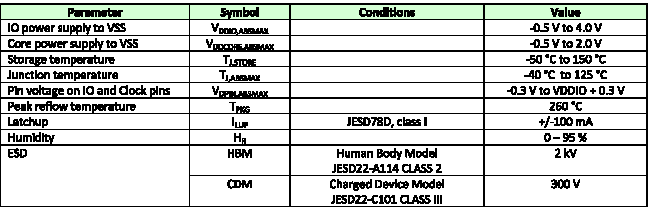
\includegraphics[width=16cm]{SX1301_table}
\caption{Caratteristiche elettriche SX1301}
\label{tab:sx1301_spec}
\end{table}
Utilizzando i valori nominali riportati nella tabella \ref{tab:sx1301_spec_1},
si hanno valori di corrente pari a 1[uA] in idle  e di 5[mA] in pieno
funzionamento.
\begin{table}[h]
\centering 
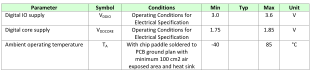
\includegraphics[width=16cm]{SX1301_table_1}
\caption{Caratteristiche elettriche SX1301}
\label{tab:sx1301_spec_1}
\end{table}
Il chip è equipaggiato con un connettore sma al quale è collegata una
antenna omindirezionale, ideata per la frequenza 868[MHz] con un guadagno pari a 3dB.
\subsection{ReliaGATE}
Il gateway a cui è collegato il modulo SX1301 è il ReliaGATE 10-11 prodotto da
Eurotech. Al suo interno troviamo un processore Texas Instruments TI AM335X Cortex-A8 
equipaggiato con 512MB di RAM e 4GB di storage eMMC. Il ReliaGATE offre una
vasta gamma di porte tra cui 232/485, 2CAN bus, 2 porte USB e 2 porte Ethernet,
inoltre ha connettività Bluetooth, WiFi e GPS. Al suo interno è installo
Everyware™ Software Framework (ESF), la versione commerciale del software Kura.
\begin{figure}[h]
\centering 
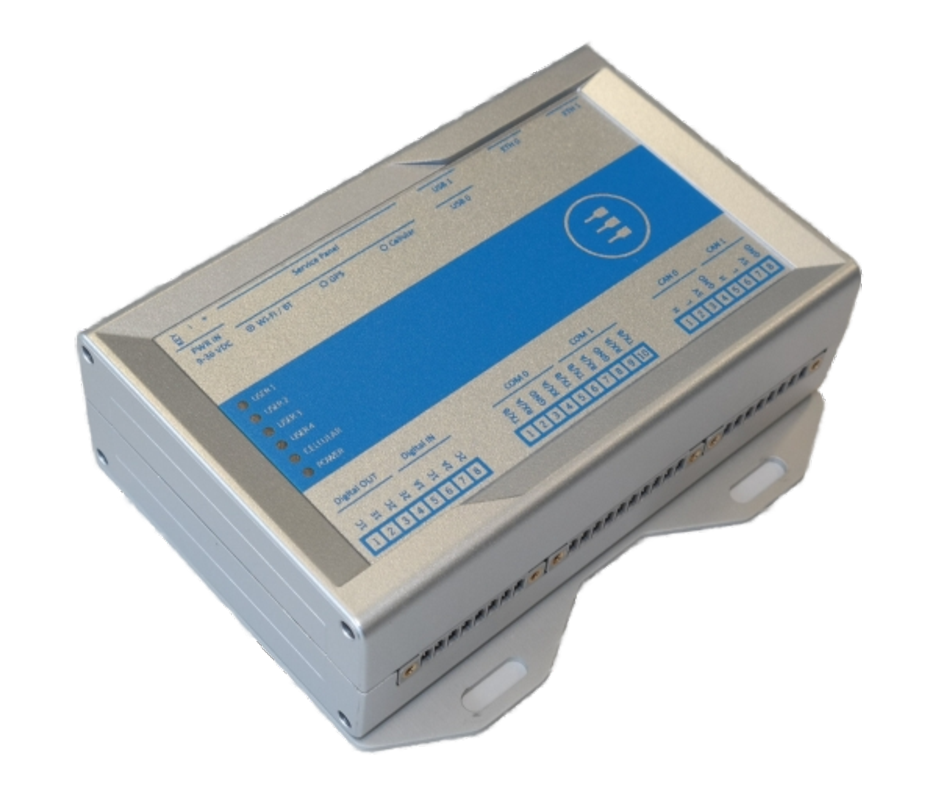
\includegraphics[width=11cm]{Reliagate_10_11}
\caption{Caratteristiche elettriche SX1301}
\label{fig:ReliaGATE}
\end{figure}


\subsection{Architettura del software}
\begin{figure}[h]
\centering 
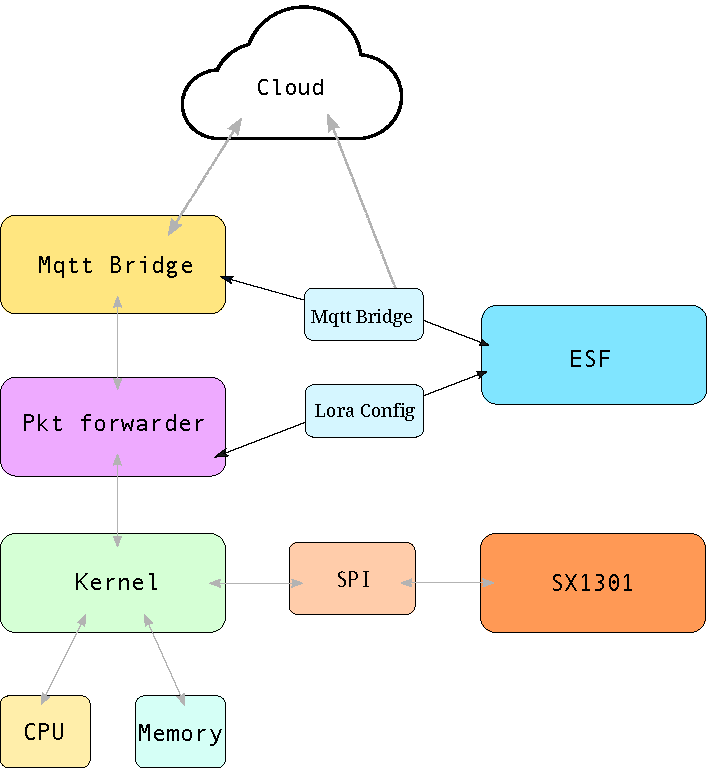
\includegraphics[width=11cm]{Application_layer}
\caption{Caratteristiche elettriche SX1301}
\label{fig:ReliaGATE}
\end{figure}

